\documentclass{article}
\usepackage{amsmath, amssymb}
\usepackage{bm}
\usepackage{graphicx} % Required for inserting images
\usepackage{tikz}
\usepackage{float}
\usepackage[round]{natbib}

\bibliographystyle{plainnat}
\usepackage[a4paper, top = 2cm,
                     bottom = 2cm,
                     left = 2cm,
                     right = 2cm]{geometry}


\title{Fences and baits : landscape connectivity in renewable resources}
\author{Simon Jean}
\date{December 2023}


%%%%%%%%%%%%%%%%%%%%%%
\newcommand*{\xMin}{0}%
\newcommand*{\xMax}{5}%
\newcommand*{\yMin}{0}%
\newcommand*{\yMax}{3}%


\newtheorem{assumption}{Assumption}

\begin{document}


\maketitle

\section*{To do :}
\begin{itemize}
\item Read Sanchirico and Wilen to check the density dependent thingy
\item Add the density dependent thingy
\item Check the jacobian properties
\item Elaborate on the dependence of future value function to the current state\textbf{s}, not only $\mathbf{X}$ but also $\mathbf{D}$ (which will eventually change $V$ through future costs ajustment, and maybe try to express decision variables as \textit{the difference between max/min connectivity and current connectivity}
\end{itemize}

\newpage

\section{Motivation}
Assume a renewable resource whose habitat spans several land patches. The resource freely flows across patches according to some biological, exogenous determinants.  Assume we have 2 patches, A and B, such that the net benefit of harvest in B is larger than in A (people in B may love the resource, while in A they just like it; they may also be more efficient at harvesting it than in A). As people in B do love their resources, they may be tempted to ensure they stay in B and fence their land. They also notice that A has resources, and are tempted to increase the migration flow from A to B, and bait the resource into B. 

In the case where both patches $A$ and $B$ value the resource, what are the policy tools that can mitigate the inflationnary loop of reciprocal fencing and baiting?

Moreover, when considering the optimal harvesting and conservation of species, conditions for patch closure to harvest depend on the residual population stock. Consider a patch closed to harvest, whose population is set to gradually recover, neighbored by an operating patch. Assume the neighboring patch can bait the resource into its patch. How should thresholds for conservation be determined in this case? 

Eventually, in the case of a invasive specious or infectious disease, how should local treatments and movement restrictions be mixed? It appears that under significant damages and lower costs, local eradication and isolation henceforth could be the economic solution, in a deterministic environment. How does that evolve with stochastic dispersal?

Overall, the question that emerges is: how does the harvest of a renewable resource change when fencing and baiting are considered?

\section{A density independent approach to endogenous dispersal}
\subsection{A 2 patch model}
In each period and each patch, the resource stock $X_{At}$ and $ X_{Bt}$ is harvested at $h_{At}$ and $h_{Bt}$, leaving a remaining stock $e_{At}$ and $ e_{Bt}$ which then grows to $g_A(e_{At})$ and $g_B(e_{Bt})$, with $g'_i()>0$ and $g''_i()<0$. Once it grows, it migrates. For example, in patch $A$, a share $d_{AAt}$ of the stock remains in $A$ in period $t$, while a share $d_{ABt} = 1-d_{AAt}$ flows from $A$ to $B$, and reciprocally for $B$. At the beginning of period $t+1$ : 
\begin{align}
    X_{At+1} = (1-d_{ABt+1})g_A(e_{At})+d_{BAt}g_B(e_{Bt})
    \\
    X_{Bt+1} = (1 - d_{BAt+1})g_B(e_{BT}) + d_{ABt}g_A(e_{At})
\end{align}

In each period, after observing the dispersal flows, landowners choose whether to improve their fences, increase the baiting, or further improve their land. 
Dispersal in the next period will depend on each landowner's fencing $z_{At}^F$and $z_{Bt}^F$ and baiting and land improvement practices $z_{At}^B$ and $z_{Bt}^B$, as well as historical dispersal $d_{ABt}$, and natural, exogenous features that limit dispersal : 
\begin{align}
    d_{ABt+1} = f_{AB}(z^F_{At}, z^B_{Bt}| d_{ABt}) \in [m_{AB},M_{AB}] \subset [0,1] \\
    d_{BAt+1} = f_{BA}(z^F_{Bt}, z^B_{At}| d_{BAt}) \in [m_{BA},M_{BA}] \subset [0,1]
\end{align}
The more one landowner fences, the more it retains the resource. However, fencing is less and less effective at retaining the resources\footnote{It may be good to go back to this hypothesis: the effect of incomplete fencing may be concave, but convex at the end when the fence is finished}. Baiting increases the flow of dispersal from the neighboring patch at a decreasing rate as well. Baiting reduces the marginal effect of fencing and fencing reduces the marginal effect of baiting.

Eventually, future dispersal depends on existing dispersal $d_{ijt}$. The larger the existing dispersal, the larger the future dispersal, with a concave effect. Conditional on $d_{ijt}$, fencing has a positive yet decreasing effect on future dispersal, and baiting incrases the flow of dispersal from a patch to its neightbor at a decreasing rate. 


 Overall : 
\begin{align*}
    \frac{\partial f_{AB}}{\partial z^F_{At}}\leq 0 &\text{ and } \frac{\partial^2 f_{AB}}{\partial (z^F_{At})^2} \geq 0\\
    \frac{\partial f_{AB}}{\partial z^B_{Bt}}\geq 0 &\text{ and } \frac{\partial^2 f_{AB}}{\partial (z^B_{Bt})^2} \leq 0\\
    \frac{\partial ^2 f_{AB}}{\partial z_{Bt}^B\partial z_{At}^F} \leq 0 &\text{ and } \frac{\partial ^2 f_{AB}}{\partial z_{At}^F\partial z_{Bt}^B} \leq 0
\end{align*}
\textbf{Add derivatives wrt to $d_{abt}$}


The timing of the model is synthetized in figure \ref{fig:timing}.

\begin{figure}[H]
  \centering
  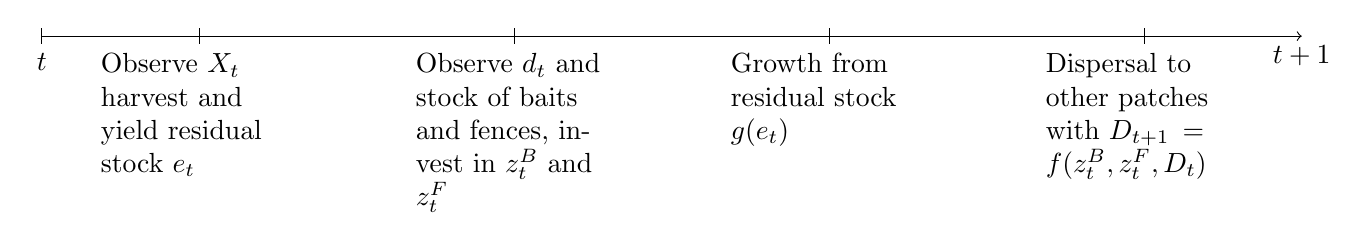
\begin{tikzpicture}
    % Draw the arrow
    \draw[->] (0,0) -- (16,0) node[anchor=north] {$t+1$};
    % Draw ticks and labels
    \draw (0, .1)--(0,-.1) node[anchor = north]{$t$};
    \draw (2, .1)--(2,-.1) node[anchor = north, text width = 2.5cm]{Observe $X_t$ harvest and yield residual stock $e_t$};
    \draw (6, .1)--(6,-.1) node[anchor = north, text width = 2.5cm] {Observe $d_t$ and stock of baits and fences, invest in $z_t^B$ and $z_t^F$};
    \draw (10, .1)--(10,-.1) node[anchor = north, text width = 2.5cm]{Growth from residual stock $g(e_t)$};
    \draw (14,.1)--(14,-.1) node[anchor = north, text width = 2.5cm]{Dispersal to other patches with $D_{t+1}=f(z_t^B, z_t^F, D_t)$};
  \end{tikzpicture}
  \caption{Timing of the model}
  \label{fig:timing}
\end{figure}


\subsection{Model formulation}
Landowners locally harvest the resource at a \textit{constant unit marginal cost} $\omega_i$ and sell it on a competitive market at price $p$, so the net marginal benefit is heterogeneous and can be written as $p_i = p - c_i$. Moreover, they choose fencing and baiting expenditures with costs $c_{i,l}(z_{it}^F)$ such that $c'_{i,l}\geq 0$ and $c''_{i,l} \geq 0$, and normalized such that $c_{i,l}(0) = 0$. The profit flow at time $t$ is
\begin{equation}
    \Pi_{it} = p_i(X_{it} - e_{it}) - c_{i,F}(z_{it}^F) - c_{i,B}(z_{it}^B)
\end{equation}

First, I'm interested in the social planner's problem, i.e, to maximize the intertemporal sum of discounted profits:
\begin{align*}
    \max_{\{e_{it}, z_{it}^F, z_{it}^B \}_{i \in \{A,B\}}} & \sum_{t=0}^T \delta^t \left( \sum_{i \in \{A,B\}} p_i(X_{it} - e_{it}) - c_{iF}(z_{it}^F) - c_{iB}(z_{it}^B) \right)\\
     &\text{Such that:}\\
        X_{At+1} &= (1-d_{ABt+1})g_A(e_{At})+d_{BAt}g_B(e_{Bt})
    \\
    X_{Bt+1} &= (1 - d_{BAt+1})g_B(e_{BT}) + d_{ABt}g_A(e_{At})\\
     d_{ABt+1} &= f_{AB}(z^F_{At}, z^B_{Bt}| d_{ABt}) \\
    d_{BAt+1} &= f_{BA}(z^F_{Bt}, z^B_{At}| d_{BAt}) 
\end{align*}
Assume each landowner can fence or bait the resource of the other into its patch, in a 2 by 2 world. What are the optimal policies? The social planner aims at maximizing : 
\begin{align*}
\max_{e_{A1}, e_{A2}, z_{A1}^F, z_{A1}^B, z_{B1}^F, z_{B1}^B}&p_A(X_{A1}-e_{A1}) - c_{AF}(z_{A1}^F) - c_{AB}(z_{A1}^B) \\
+ &p_B(X_{B1}-e_{B1}) - c_{BF}(z_{B1}^F) - c_{BB}(z_{B1}^B) \\
+ & \delta \left(p_A((1-f_{AB}(z_{A1}^F, z_{B1}^B, d_{AB1}))g_A(e_{A1}) + f_{BA}(z_{B1}^F, z_{A1}^B, d_{BA1})g_B(e_{B1}))\right.\\
& + \left. p_B((1-f_{BA}(z_{B1}^F, z_{A1}^B, d_{BA1}))g_B(e_{B1}) + f_{AB}(z_{A1}^F, z_{B1}^B, d_{AB1})g_A(e_{A1})) \right)
\end{align*}
\subsection{First order conditions for interior solutions}
For an interior solution to emerge, the following FOCs need to hold. 
The optimal escapement FOCs are : 
\begin{align}
&\frac{p_A}{\delta \left(p_A + f_{AB}(z_{A1}^F, z_{B1}^B, d_{AB1})(p_B-p_A)\right)} = g_A'(e_{A1}) \label{eq:ea1}\\
%
&\frac{p_B}{\delta \left( p_B + f_{BA}(z_{B1}^F, z_{A1}^B, d_{BA1})(p_A-p_B)\right)} = g_B'(e_{B1}) \label{eq:ea2}
\end{align}
And the optimal fencing and baiting FOCs are:
\begin{align}
c'_{AF}(z_{A1}^F) &= \delta g_A(e_{A1}) \frac{\partial f_{AB}(z_{A1}^F, z_{B1}^B, d_{AB1})}{\partial z_{A1}^F}\left(p_B - p_A \right) \label{eq:zaf1}\\
%
c'_{BF}(z_{B1}^F) &= \delta g_B(e_{B1}) \frac{\partial f_{BA}(z_{B1}^F, z_{A1}^B, d_{BA1})}{\partial z_{B1}^F}(p_A - p_B) \label{eq:zbf1}\\
%
c'_{AB}(z_{A1}^B) &= \delta  g_B(e_{B1})\frac{\partial f_{BA}(z_{B1}^F, z_{A1}^B, d_{BA1})}{\partial z_{A1}^B}(p_A - p_B) \label{eq:zab1}\\
%
c'_{BB}(z_{B1}^B) & = \delta g_A(e_{A1}) \frac{\partial f_{AB}(z_{A1}^F, z_{B1}^B, d_{AB1})}{\partial z_{B1}^B}(p_{B} - p_{A})
\label{eq:zbb1}
\end{align}
In this context, an interior solution means (i) positive escapement in patches $A$ and $B$ (e.g $e_{i1}>0$), (ii) positive spending in fencing and baiting (e.g. $z_{i1}^k$ with $k \in \{B, F\}$) in patches $A$ and $B$ and (iii) spending in fencing and baiting is not constrained by a maximum in patches $A$ and $B$. 
\\
\subsection{A homogeneous distribution of net marginal benefits yield a state independent, golden-rule solution}
 Consider the case where resources are as valuable in both patches $p_B = p_A$. In this case, equations \ref{eq:zaf1}, \ref{eq:zbf1}, \ref{eq:zab1}, \ref{eq:zbb1} imply no investment in either fencing nor baiting is optimal. In this case, the solution collapses back to the golden rule of renewable resource harvesting, where 
\begin{align*}
z_{A1}^B =& z_{A1}^F = 0\\
z_{B1}^B =& z_{B1}^F = 0\\
g'_A(e_{A1}) &= \frac{1}{\delta}\\
g'_B(e_{B1}) &= \frac{1}{\delta}
\end{align*}

\subsection{A heterogeneous distribution of net marginal benefits yields an??}

Now assume $p_A \neq p_B$ (and for the sake of exposition $p_B > p_A$). Remember that fencing \textit{reduces} dispersal outflow, and baiting \textit{increases} dispersal outflow (e.g. $\frac{\partial f_{AB}}{\partial z_{A1}^F}<0$, $\frac{\partial f_{AB}}{\partial z_{B1}^B}>0$ and reciprocally). Equations \ref{eq:zaf1} and \ref{eq:zab1} show that no investing  in fencing and baiting in $A$ is optimal, as the right hand side is negative. Investing in fencing and baiting is only efficient in $B$ (eq. \ref{eq:zbf1}, \ref{eq:zbb1}). This conforms with economic intuition : if there is an arbitrage opportunity between two locations, it is optimal to leverage it as much as economically possible.

Therefore, no fully interior solution emerges in the optimal 2 patch 2 periods case. \\\\

The optimal solution therefore collapses to : 
\begin{align*}
g_A'(e_{A1}) &= \frac{p_A}{\delta \left(p_A + f_{AB}(0, z_{B1}^B, d_{AB1})(p_B-p_A)\right)} \\
%
g_B'(e_{B1}) &= \frac{p_B}{\delta \left( p_B + f_{BA}(z_{B1}^F, 0, d_{BA1})(p_A-p_B)\right)} \\
%
c'_{BF}(z_{B1}^F) &= \delta g_B(e_{B1}) \frac{\partial f_{BA}(z_{B1}^F, 0, d_{BA1})}{\partial z_{B1}^F}(p_A - p_B)\\
%
c'_{BB}(z_{B1}^B) & = \delta g_A(e_{A1}) \frac{\partial f_{AB}(0, z_{B1}^B, d_{AB1})}{\partial z_{B1}^B}(p_{B} - p_{A})
\end{align*}

First, while the equations governing the optimal escapement in patch $A$ and $B$ resemble Costello and Polasky (2008) in an exogenous dispersal framework, they substantially differ as $e_{A1}^*, e_{B1}^*, z_{B1}^{B*}, z_{B1}^{F*}$ are jointly determined, and are therefore \textit{not state independent}, as they depend on $d_{AB1}$.

Second, the stocks must be harvested down to the point where the current forgone net marginal benefit equals the discounted future marginal benefits at the social scale, that is, the marginal value of the units remaining in the own patch and of the units \textit{endogenously} migrating to the other patch. A \textit{golden rule} type of solution can emerge in the case where $f_{AB}()= f_{AB}()=0$ and $\frac{\partial f_{AB}}{\partial z_{B1}^F} = \frac{\partial f_{AB}}{\partial z_{B1}^B}=0$, that is to say when there is no spatial process.

Third, the optimal allocation between fencing and baiting is such that the actualized, productivity weighted, per resource unit, marginal cost of each options are equalized: 

$$
\frac{c'_{BF}(z_{B1}^F)}{- \frac{\partial f_{BA}(z_{B1}^F, 0, d_{BA1})}{\partial z_{B1}^F}}\frac{1}{\delta g_{B}(e_{B1})} = \frac{c'_{BB}(z_{B1}^B)}{- \frac{\partial f_{AB}(0, z_{B1}^B, d_{AB1})}{\partial z_{B1}^B}}\frac{1}{\delta g_{A}(e_{A1})}
$$
The intuition is straightforward : the social planner invests in either option until the point where the discounted marginal benefit of increasing (resp. decreasing) the inflow (resp. the outflow) of the resource in (resp. outside) the patch equals its cost.

Eventually, it is not clear how fencing and baiting relate to optimal escapement in the social optimum (the comparative statics are ugly to derive)
\begin{enumerate}
\item Find the total derivative of each line
\item Find the number of derivatives we want to get
\item Put the problem in the Cramer's rule form and Jacobian analysis

Finally, note that the first order conditions for $e_{A1}^*$ and $z_{B1}^{B*}$ for an independent system from the FOCs determining $e_{B1}^*$ and $z_{B1}^{B*}$. Therefore, we can analyze the joint system with two independent subsystems. Moreover, given the partially corner solution, we can reframe dispersal, as a dimension is fixed, as a 2 dimension, additive process: $f_{AB}(0, z_{B1}^B; d_{AB1}) \equiv \omega_d(d_{AB1}) + \omega_z \left(z_{B1}^B \right)$, and $f_{BA}(z_{B1}^F, 0 ; d_{BA1}) \equiv \psi_d(d_{BA1}) + \psi_z \left(z_{B1}^B \right)$ such that $\psi_z'()<0, \psi_z''()>0$ and $\omega_z'()>0, \omega_z''()<0$ (see figure 2), and $\omega_d'()>0$ and $\Psi_d'()>0$

In the appendix \ref{sec:jacobian}, I derive the comparative statics of the implicit functions defined by the two subsystems relating $e_{A1}$ and $z_{B1}^B$; and $e_{B1}$ and $z_{B1}^F$.

\begin{figure}
	\label{fig:additive_dispersal}
	\begin{center}
		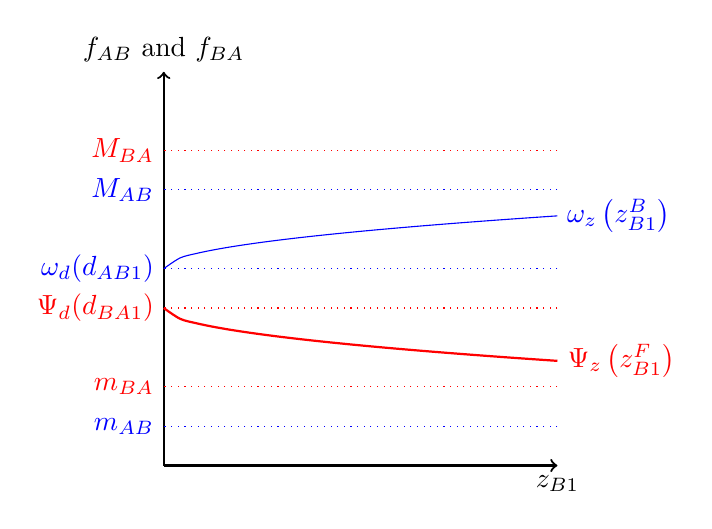
\begin{tikzpicture}
    % Draw grid
    \draw[thick, ->, black](0,0) -- (0,5) node[anchor = south]{$f_{AB}$ and $f_{BA}$};
    \draw[thick, ->, black](0,0) -- (5,0) node[anchor = north]{$z_{B1}$};
    % Draw horizontal lines
    \draw[dotted, red] (5,4) -- (0,4) node[anchor=east]{$M_{BA}$}; % y=8 line
    \draw[dotted, red] (5,1) -- (0,1) node[anchor=east]{$m_{BA}$}; % y=1 line
    % Draw the curve
    \draw[dotted, red](5,2) -- (0,2) node[anchor = east]{$\Psi_d(d_{BA1})$};
    \draw[thick,red,smooth] plot[domain=0:5] (\x,{2 - 0.3*\x^0.5}) node[anchor = west]{$\Psi_z\left(z_{B1}^F\right)$};
     \draw[blue,smooth] plot[domain=0:5] (\x,{2.5 + 0.3*\x^0.5}) node[anchor = west]{$\omega_z\left(z_{B1}^B\right)$};
     \draw[dotted, blue](5,2.5) -- (0,2.5) node[anchor = east]{$\omega_d(d_{AB1})$};
    \draw[dotted, blue] (5,3.5) -- (0,3.5) node[anchor=east]{$M_{AB}$}; % y=8 line
    \draw[dotted, blue] (5,.5) -- (0,.5)node[anchor=east]{$m_{AB}$};
    % Note: Adjust the function inside the plot command to get the desired curve shape

		\end{tikzpicture}
		\caption{Dispersal with partially corner solution}
	\end{center}
\end{figure}



\end{enumerate}
\section*{Annex}
\subsection{Subsystems analysis : comparative statics}
\label{sec:jacobian}
\subsubsection{Optimal escapement and fencing in patch $B$}
Using equations \ref{eq:ea2} and \ref{eq:zbf1} to define a set of implicit solutions : 
\begin{align*}
g'_B(e_{B1}) \delta \left( p_B + (\Psi_z(z_{B1}^F) + \Psi_d(d_{BA1})\right)(p_A - p_B) - p_A &= 0\\
%
c'_{BF}(z_{B1}^F) - \delta g_B(e_{B1}) \Psi_z'(z_{B1}^F)(p_A -p_B)&=0
\end{align*}
Taking total differential : 
\begin{align*}
g''_B(e_{B1})\delta \left[p_B + \Psi_z(z_{B1}^F) + \Psi_d(d_{BA1})(p_A-p_B)\right] de_{B1} + g_B'(e_{B1}) & \delta (p_A - p_B)\left( \Psi_z'(z_{B1}^F)dz_{b1}^F + \Psi_d'(d_{BA1})d(d_{BA1}) \right) = 0\\
\left(c''_{BF}(z_{B1}^F) - \delta g_B(e_{B1})\Psi''_z(z_{B1}^F)(p_A - p_B)\right) dz_{B1}^F & - \delta g'_B(e_{B1}) \Psi_z(z_{B1}^F)(p_A-p_B)de_{B1}=0
\end{align*}

And put in matrix form
\begin{equation*}
\begin{bmatrix}
g''_B(e_{B1}) \delta \left(p_B + (\Psi_z(z_{B1}^F) \right. & \delta g'_B(e_{B1})(p_A - p_B)  \\
%
\left. + \Psi_d(d_{BA1}))(p_A-p_B) \right) & \times \Psi'_z(z_{B1}^F)
\\
\\
 - \delta g_B'(e_{B1}) & c''_{BF}(z_{B1}^F) - \delta g_B(e_{B1}) \\
\times (p_A - p_B)\Psi_z'(z_{B1}^F) & \times \Psi''_z(z_{B1}^F)(p_A - p_B)
\end{bmatrix} 
\times
\begin{bmatrix}
de_{B1}\\
dz_{B1}^F
\end{bmatrix} = 
\begin{bmatrix}
(p_B - p_A) \delta g'_B(e_{B1})\Psi_d'(d_{BA1})\\
0
\end{bmatrix}
d(d_{BA1})
\end{equation*}
Let the determinant of the above Jacobian matrix be $det(J) = J_{11}J_{22} - J_{12}J_{21}$ with
\begin{align*}
J_{11} & = g''(e_{B1})\delta \left( p_B + (\Psi_z(z_{B1}^F) + \Psi_d(d_{BA1}))(p_A - p_B)\right) <0 \\
J_{12} & =  g'_{B}(e_{B1})\delta (p_A - p_B) \Psi_z'(z_{B1}^F) >0 \\
J_{21} & = - J_{12} <0 \\
J_{22} & = c''_{BF}(z_{B1}^F) - \delta g_B(e_{B1})(p_B - p_A) \Psi''_z(z_{B1}^F)
\end{align*}
\textbf{Issue with the computation of the Jacobian and the conditions. }
 \begin{itemize}
 \item If $J_{22} < 0$, then $|J|>0$
 \item if $J_{22} >0$ and $J_{12}J_{21}>J_{11}J_{22}$, then $|J|>0$
 \item if not, $|J|<0$. 
 \end{itemize}
$\Rightarrow$ A wide array of results emerge, but under mild conditions, intuitive results arise (eg, stock remaining increases in existing dispersal), investment decreases in existing dispersal, and investment and stock are substitutes
\subsection{Infinite horizon}
In this section, I formulate the problem in a recursive framework, and adopt a resolution approach assuming the value function exists, to characterize the main mechanisms. 
\subsubsection{Value function}
Given the dynamic nature of the problem, a Bellman equation can be formulated: 
\begin{equation}
\begin{aligned}[b]
V(\mathbf{X_t,D_t}) &= \max_{ \{e_{it}, z_{it}^F, z_{it}^B\}_{i \in A,B} } \sum_{i \in \{A,B\}} \left( p_i(X_{it} - e_{it}) - c_{iF}(z_{it}^F) - c_{iB}(z_{it}^B) \right)+ \delta V\left(\mathbf{X_{t+1}, D_{t+1}}\right)\\
& = \max_{ \{e_{it}, z_{it}^F, z_{it}^B\}_{i \in A,B} } \sum_{i \in \{A,B\}} \left(p_i(X_{it} - e_{it}) - c_{iF}(z_{it}^F) - c_{iB}(z_{it}^B) \right) + \delta V(\mathbf{D_{t+1}g(e_t)})\\
&= \max_{ \{e_{it}, z_{it}^F, z_{it}^B\}_{i \in A,B} } \sum_{i \in \{A,B\}} \left( p_i(X_{it} - e_{it}) - c_{iF}(z_{it}^F) - c_{iB}(z_{it}^B)\right) + \delta V\left(X_{At+1}; X_{Bt+1} \right)
\end{aligned}
\end{equation}
Where $X_{t+1}^A = (1-f_{AB}(z^F_{At}, z^B_{Bt}| d_{ABt}))g_A(e_{At})+f_{BA}(z^F_{Bt}, z^B_{At}| d_{BAt})g_B(e_{Bt})$\\

and $X_{t+1}^B =(1 - f_{BA}(z^F_{Bt}, z^B_{At}| d_{BAt}))g_B(e_{BT}) +f_{AB}(z^F_{At}, z^B_{Bt}| d_{ABt})g_A(e_{At})$

\subsubsection{First order conditions}
The necessary conditions for interior solutions to hold are :

\begin{align}
\frac{\partial V}{\partial e_{At}} =  0 &\iff - p_A + \delta g'_A(e_{At})\left( \frac{\partial V}{\partial X_{At+1}} + f_{AB}(z_{At}^F, z_{Bt}^B; d_{ABt})\left[\frac{\partial V}{\partial X_{Bt+1}} - \frac{\partial V}{\partial X_{At+1}} \right] \right)=0 \label{eq:foc_eat}\\
%
\frac{\partial V}{\partial e_{Bt}} =  0 &\iff - p_B + \delta g'_B(e_{Bt})\left( \frac{\partial V}{\partial X_{Bt+1}} + f_{BA}(z_{Bt}^F, z_{At}^B; d_{BAt})\left[\frac{\partial V}{\partial X_{At+1}} - \frac{\partial V}{\partial X_{Bt+1}} \right] \right) = 0 \label{eq:foc_ebt}\\
%
\frac{\partial V}{\partial z^F_{At}} = 0 &\iff -c'_{AF}(z_{At}^F) + \delta g_A(e_{At}) \frac{\partial f_{AB}(z_{At}^F, z_{Bt}^B, d_{ABt})}{\partial z_{At}^F} \left[\frac{\partial V}{\partial X_{Bt+1}} - \frac{\partial V}{\partial X_{At+1}}  \right] = 0\label{eq:foc_zfa}\\
%
\frac{\partial V}{\partial z^F_{Bt}} = 0 &\iff -c'_{BF}(z_{Bt}^F) + \delta g_B(e_{Bt}) \frac{\partial f_{BA}(z_{Bt}^F, z_{At}^B, d_{BAt})}{\partial z_{Bt}^F} \left[\frac{\partial V}{\partial X_{At+1}} - \frac{\partial V}{\partial X_{Bt+1}}  \right] = 0\label{eq:foc_zfb}\\
%
\frac{\partial V}{\partial z_{At}^B} = 0 &\iff - c'_{AB}(z_{At}^B) + \delta g_B(e_{Bt}) \frac{\partial f_{BA}(z_{Bt}^F, z_{At}^B, d_{BAt})}{\partial z_{At}^B} \left[ \frac{\partial V}{\partial X_{At+1}} - \frac{\partial V}{\partial X_{Bt+1}}\right] = 0 \label{eq:foc_zba}\\
%
\frac{\partial V}{\partial z_{Bt}^B} = 0 &\iff - c'_{BB}(z_{Bt}^B) + \delta g_A(e_{At}) \frac{\partial f_{AB}(z_{At}^F, z_{Bt}^B, d_{ABt})}{\partial z_{Bt}^B} \left[ \frac{\partial V}{\partial X_{Bt+1}} - \frac{\partial V}{\partial X_{At+1}}\right] = 0
\label{eq:foc_zbb}
\end{align}


Under this set of assumptions, the system can be rewritten as : 
\begin{align}
p_A &= \delta g'_A(e_{At}) \left(\frac{\partial V}{\partial X_{At+1}} + f_{AB}(0, z_{Bt}^B; d_{ABt})\left[\frac{\partial V}{\partial X_{Bt+1}} - \frac{\partial V}{\partial X_{At+1}}  \right] \right)\\
%
p_B &= \delta g'_B(e_{Bt}) \left(\frac{\partial V}{\partial X_{Bt+1}} + f_{BA}(z_{Bt}^F, 0; d_{BAt})\left[\frac{\partial V}{\partial X_{At+1}} - \frac{\partial V}{\partial X_{Bt+1}}  \right] \right)\\
%
\frac{c'_{BF}(z_{Bt}^F)}{\frac{\partial f_{BA}(z_{Bt}^F, 0; d_{BAt})}{\partial z_{Bt}^F}} &= \delta g_B(e_{Bt})\left[ \frac{\partial V}{\partial X_{At+1}} - \frac{\partial V}{\partial X_{Bt+1}} \right]\\
%
\frac{c'_{BB}(z_{Bt}^B)}{\frac{\partial f_{AB}(0, z_{Bt}^B; d_{ABt})}{\partial z_{Bt}^B}} &= \delta g_A(e_{At})\left[ \frac{\partial V}{\partial X_{Bt+1}} - \frac{\partial V}{\partial X_{At+1}} \right]
\end{align}
Several comments are in order. First, it appears that if an interior solution exists, it is not \textit{state independent} (see \cite{costello_optimal_2008}). Contrary to \cite{costello_optimal_2008}, optimal escapement does not depend on exogenous dispersal parameters. Current dispersal is endogenously chosen, given the past dispersal. As the decision variables are co-determined, and fencing and baiting depend on past connectivity, the solution cannot be fully \textit{ state independent}. In the special case where dispersal is a contemporaneous choice and there is no dependence on the past, the solution would be fully \textit{state independent}.
Notice however that the solution seems \textbf{partially} state-independent. 
%As a matter of fact, while all the choice variables depend on the past observed dispersal, for $e_{it} \in ]0,X_{it}[$, $e_{it}$ does not depend on $X_{it}$, but depends on $\mathbf{D}_t$.
 If past dispersal from $A$ to $B$ is already large, for example, patch $B$ will limit its investment in baiting. As a result, it will modify its harvest rules, and while $e_{it}$ will not depend on the observed remaining quantities, it will depend on the observed dispersal. 

Second, the resource in patch $A$ must be harvested down to the point where the forgone revenue of 1 extra unit of harvest ($p_A$) equals the discounted future marginal revenue of letting it escape. In this case, it is equal to the value of the share of the resource that remains in $A$ and that \textit{endogenously} migrates to $B$. A similar reasoning explains the optimal escapement in $B$. 

Third, the productivity weighted marginal cost of fencing in $B$ equals the discounted future value of keeping the resource in $B$ rather than in $A$. The productivity weighted marginal cost of baiting equals the discounted future of value of baiting the resource from $A$ to $B$. If the marginal productivity of fencing (or baiting) tends to 0 when fencing (or baiting) tends to infinity for all observed dispersals, then optimal interior solutions exist, and marginal revenues are equalized across options, each option must be carried on until its marginal cost equals the future arbitrage between $A$ and $B$.  Fencing and baiting are such that the actualized, productivity weighted marginal cost of fencing per unit of future resource in $B$ equals the actualized productivity weighed marginal cost of baiting per unit of future resource in $A$, and they both equal the arbitrage between $B$ and $A$ in $t+1$ : 

$$
\frac{c'_{BF}(z_{Bt}^F)}{-\frac{\partial f_{BA}(z_{Bt}^F, 0; d_{BAt})}{\partial z_{Bt}^F}} \frac{1}{\delta} \frac{1}{g_B(e_{Bt})} = \frac{c'_{BB}(z_{Bt}^B)}{\frac{\partial f_{AB}(0, z_{Bt}^B; d_{ABt})}{\partial z_{Bt}^B}} \frac{1}{\delta} \frac{1}{g_A(e_{At})}
$$

Fourth, it is clear that escapement and fencing and baiting are mutually dependent. To be clearer, escapement in patch $B$ and fencing in $B$ are related, while escapement in $A$ and baiting in $B$ are related. 
\subsubsection{Discussion and questions}
\begin{itemize}
\item Corner solutions do not rely too much on the constant marginal benefits of harvest. The limiting factor for fencing and baiting here is the cost of each action. With a decreasing marginal benefit of harvest, an additional discounted limiting factor would most likely reduce baiting and fencing, but still yield a partially corner solution. In this case, the solution would likely equalize the marginal benefit of harvest in $A$ absent investment to the marginal benefit of harvest in $B$ with optimal fencing and baiting. 

\item The dependence of the residual stock on $\mathbf{D}_t$, and therefore of $X_{t+1}$ on $\mathbf{D}_t$ questions how to interpret the derivative $\frac{\partial V}{\partial X_{it+1}}$. On the one hand, by including the detailed law of motion of $\mathbf{X}_t$ with endogenous dispersal, the differential disentangles effects of changes in fencing, baiting and harvesting. However, something may be wrong with the formulation of the problem here : the effect of a change in dispersal tomorrow is not only the sum of price effects across space, but also changes in costs of fencing and baiting as these decisions depend on dispersal. It seems there may be a piece missing, by not measuring the \textit{direct} value effects of a change in dispersal.\\
$\Rightarrow$ Is it worth looking into an other formulation such as $V(\mathbf{X}_{t+1}, \mathbf{D}_{t+1}) = V(\mathbf{D}_{t+1}g(\mathbf{e}_t), \mathbf{D}_{t+1})$. This would push the problem to evaluate the derivative wrt the second argument, but could maybe disentangle the effects and leverage 'partial' state independence?.
%\item One way to have state independence maybe can be to (i) reformulate the problem using $V(\mathbf{D}_{t+1}g(\mathbf{e}_t), \mathbf{D}_{t+1})$ and (ii) impose a \textbf{constant marginal cost} of investment in fencing or baiting as well as (iii) 
\item \cite{costello_optimal_2008} hinges on the "escapement trick" : is there something akin that can be found for dispersal? Can I reframe the choice of future dispersal as a choice within bounds like $M_i$ and $d_{ABt}$ arguing that if a solution is interior, it is state independent? 
\end{itemize}
\subsection{Calibration}
In order to gain further insights, I calibrate a fictitious model between patches $A$ and $B$. 

%First, dispersal between $A$ and $B$ is of the form :
%\begin{equation}
%d_{ABt+1} = m_{AB} +  \frac{M_{AB} - m_{AB}}{1+ \exp(-((z_{At}^F)^\kappa - (z_{Bt}^B)^\nu + \beta d_{ABt}))}
%\end{equation}
%This functional form is bounded, decreases with $z_{At}^F$ and increases with $z_{Bt}^B$, and allows for a potential decay of connectivity through time.

%Need to change so that : if $z_{At}^F= z_{Bt}^B = 0$, $d_{ABt+1} = \beta d_{ABt}$, does not work. 

\subsubsection{Dispersal}
Dispersal needs to be such that : 
\begin{itemize}
\item if $z_{At}^F = z_{Bt}^B - 0$, then $d_{ABt+1}=\beta d_{ABt}$
\item Be bounded between $m_{AB}$ and $M_{AB}$
\item Increasing in baiting, and decreasing in fencing
\item Different productivities of fencing and baiting determine the overall flow

\item Would be interesting if it can be grounded in some ecological theory, but beyond just density dependent (or how density dependence can be amended).
\end{itemize}
$\Rightarrow$ look into a logit function
\end{document}
